%--------------------------
%Hiperbolóide
%--------------------------

\begin{figure}[H]
  \centering
  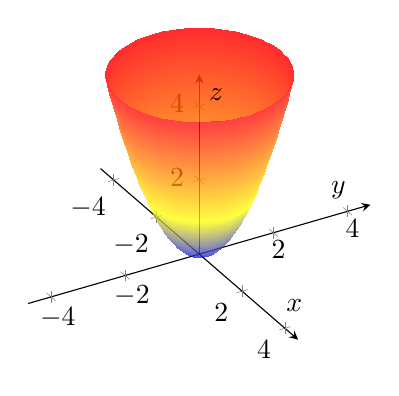
\begin{tikzpicture}
    \begin{axis}[
      view={60}{30},
      axis lines=middle,
      xlabel={$x$}, ylabel={$y$}, zlabel={$z$},
      domain=0:360,          % theta em graus
      y domain=0:2.2,        % r (raio) -> ajuste aqui
      samples=80,
      samples y=35,
      z buffer=sort,
      grid=major,
      axis equal,
    ]

      % 1) "Sino" (parabolóide) com domínio circular
      \addplot3[
        surf,
        shader=interp,
        opacity=0.75,
        draw=none             % tira as linhas da malha (fica mais "GeoGebra")
      ]
      (
        {y*cos(x)},           % x = r cos(theta)
        {y*sin(x)},           % y = r sin(theta)
        {y^2}                 % z = r^2
      );

      % 2) "Boca plana": disco no topo z = R^2
      %    (usa o MESMO R do y domain máximo)
      \addplot3[
        surf,
        shader=interp,
        opacity=0.30,
        draw=none
      ]
      (
        {y*cos(x)},
        {y*sin(x)},
        { (2.2)^2 }           % <-- aqui: R^2 (tem que bater com o y domain máximo)
      );

    \end{axis}
  \end{tikzpicture}
\end{figure}